\documentclass[11pt,a4paper]{article}
\usepackage[margin=2.3cm]{geometry}
\usepackage{amsmath,amssymb}
\usepackage{graphicx}
\usepackage{booktabs}
\usepackage{array}
\usepackage{xcolor}
\usepackage{enumitem}
\usepackage[font=small,labelfont=bf]{caption}
\usepackage[most]{tcolorbox}
\usepackage{tikz}
\usetikzlibrary{arrows.meta,positioning,shapes.geometric,calc,decorations.pathreplacing,patterns,fit,backgrounds}
\usepackage[colorlinks=true,linkcolor=blue!50!black,urlcolor=blue!50!black]{hyperref}

\definecolor{bird}{RGB}{250,190,45}
\definecolor{scalec}{RGB}{51,140,230}
\definecolor{feeder}{RGB}{230,77,64}
\definecolor{teach}{RGB}{106,61,154}
\definecolor{stud}{RGB}{27,158,119}
\definecolor{warn}{RGB}{215,48,39}

\tikzset{
  box/.style={draw, rounded corners=3pt, align=center, minimum height=1.0cm, text width=2.6cm, font=\small, fill=white},
  data/.style={box, fill=gray!10},
  model/.style={box, fill=teach!12, draw=teach},
  geo/.style={box, fill=bird!20, draw=bird!70!black},
  res/.style={box, fill=stud!15, draw=stud},
  arr/.style={-{Stealth[length=2.6mm]}, thick},
}
\newtcolorbox{keybox}[1][]{colback=teach!5, colframe=teach!70!black, fonttitle=\bfseries, title=#1, sharp corners=south}
\newtcolorbox{notebox}[1][]{colback=warn!4, colframe=warn!70!black, fonttitle=\bfseries, title=#1, sharp corners=south}

\title{\textbf{Estimating broiler weight from overhead video}\\[2pt]
\large Methodology of the \texttt{broilerseg} package: segmentation, calibration,\\ the slice-volume model, the fitted mass equation and its validation}
\author{Prepared for Grace Akintan}
\date{\today}

\begin{document}
\maketitle
\tableofcontents
\vspace{1em}

% =========================================================================
\section{The pipeline at a glance}
% =========================================================================
A camera looks straight down on a weighing scale. A feeding pan of known size sits on the scale. Each time a broiler steps onto the scale, FlockLabel records the scale reading for every labelled video frame. The package turns each frame into a weight estimate in five stages (Figure~\ref{fig:pipeline}) and checks it against those scale readings.

\begin{figure}[h]
\centering
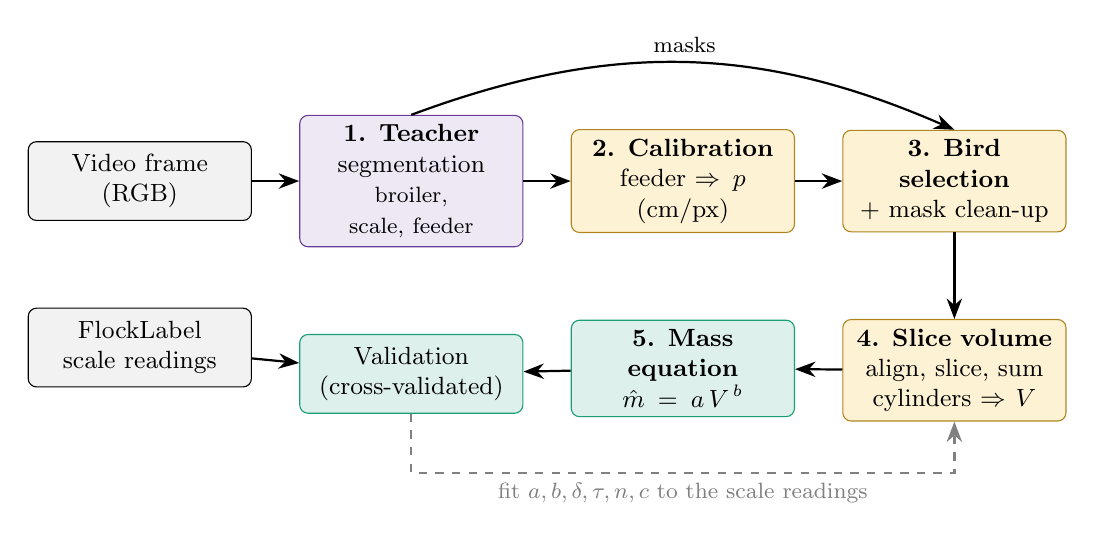
\begin{tikzpicture}[node distance=0.55cm and 0.6cm]
  \node[data] (vid) {Video frame\\(RGB)};
  \node[model, right=of vid] (seg) {\textbf{1. Teacher}\\segmentation\\{\footnotesize broiler, scale, feeder}};
  \node[geo, right=of seg] (cal) {\textbf{2. Calibration}\\feeder $\Rightarrow p$ (cm/px)};
  \node[geo, right=of cal] (sel) {\textbf{3. Bird selection}\\+ mask clean-up};
  \node[geo, below=1.1cm of sel] (vol) {\textbf{4. Slice volume}\\align, slice, sum\\cylinders $\Rightarrow V$};
  \node[res, below=1.1cm of cal] (mass) {\textbf{5. Mass equation}\\$\hat m = a\,V^{\,b}$};
  \node[res, below=1.1cm of seg] (eval) {Validation\\(cross-validated)};
  \node[data, below=1.1cm of vid] (gt) {FlockLabel\\scale readings};
  \draw[arr] (vid) -- (seg);
  \draw[arr] (seg) -- (cal);
  \draw[arr] (cal) -- (sel);
  \draw[arr] (seg.north) to[bend left=22] node[above, font=\footnotesize]{masks} (sel.north);
  \draw[arr] (sel) -- (vol);
  \draw[arr] (vol) -- (mass);
  \draw[arr] (mass) -- (eval);
  \draw[arr] (gt) -- (eval);
  \draw[arr, dashed, gray] (eval.south) -- ++(0,-0.75) -| node[pos=0.25, below, font=\footnotesize, text=gray]{fit $a, b, \delta, \tau, n, c$ to the scale readings} (vol.south);
\end{tikzpicture}
\caption{Overview. Stages 1--4 are geometry; stage 5 holds the parameters that are fitted to the scale readings (dashed arrow). Notebook~1 runs stages 1--5 with the large teacher model; Notebook~2 trains a small YOLO student to replace stage~1 on a Raspberry Pi (Section~\ref{sec:distill}).}
\label{fig:pipeline}
\end{figure}

% =========================================================================
\section{Stage 1 -- Segmentation with a text-prompted teacher}
% =========================================================================
The teacher turns short text phrases into pixel masks, so no masks have to be drawn by hand. Two interchangeable teachers are available:

\begin{itemize}[nosep]
  \item \textbf{Grounded SAM 2} (default; public, Apache-2.0): Grounding DINO turns each phrase into \emph{boxes}, then SAM~2.1 draws a \emph{mask} inside every box (Figure~\ref{fig:grounded}).
  \item \textbf{SAM 3} (gated): detection and masks come from one model.
\end{itemize}

\begin{figure}[h]
\centering
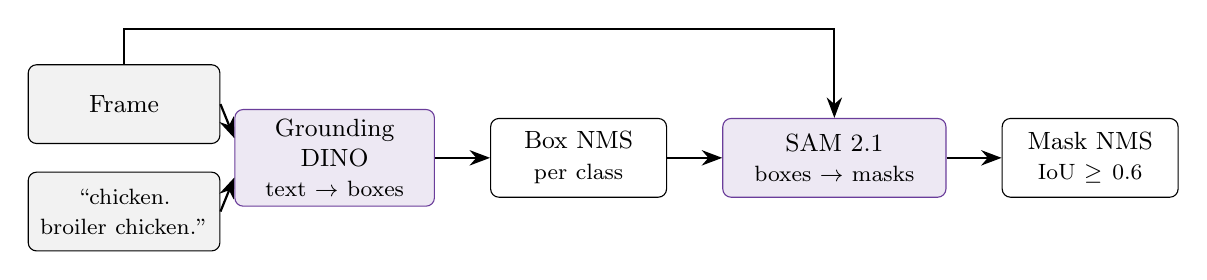
\begin{tikzpicture}[node distance=0.5cm and 0.7cm]
  \node[data, text width=2.2cm] (img) {Frame};
  \node[data, below=0.35cm of img, text width=2.2cm] (txt) {\footnotesize ``chicken.\\ broiler chicken.''};
  \node[model, right=1.4cm of $(img)!0.5!(txt)$, text width=2.3cm] (dino) {Grounding DINO\\{\footnotesize text $\to$ boxes}};
  \node[box, right=of dino, text width=2.0cm] (nms) {Box NMS\\{\footnotesize per class}};
  \node[model, right=of nms] (sam) {SAM 2.1\\{\footnotesize boxes $\to$ masks}};
  \node[box, right=of sam, text width=2.0cm] (mnms) {Mask NMS\\{\footnotesize IoU $\ge 0.6$}};
  \draw[arr] (img.east) -- ($(dino.west)+(0,0.25)$); \draw[arr] (txt.east) -- ($(dino.west)+(0,-0.25)$);
  \draw[arr] (dino) -- (nms); \draw[arr] (nms) -- (sam); \draw[arr] (sam) -- (mnms);
  \draw[arr] (img.north) -- ++(0,0.45) -| (sam.north);
\end{tikzpicture}
\caption{Grounded SAM 2. Each class (broiler, scale, feeder) has its own text query. Overlapping duplicates are removed first as boxes, then as masks.}
\label{fig:grounded}
\end{figure}

\paragraph{Which bird is on the scale?} Several broilers can be visible. During validation, the broiler whose box best overlaps the FlockLabel box is chosen (highest box IoU). Without a box (deployment), the bird with the largest share of its mask over the \emph{platform region} is chosen. That region is the filled convex hull of the scale and feeder masks. The convex hull is needed because the bird hides part of the scale it stands on (Figure~\ref{fig:select}). The chosen mask is then cleaned: a small opening removes specks, only the largest blob is kept, and holes are filled.

\begin{figure}[h]
\centering
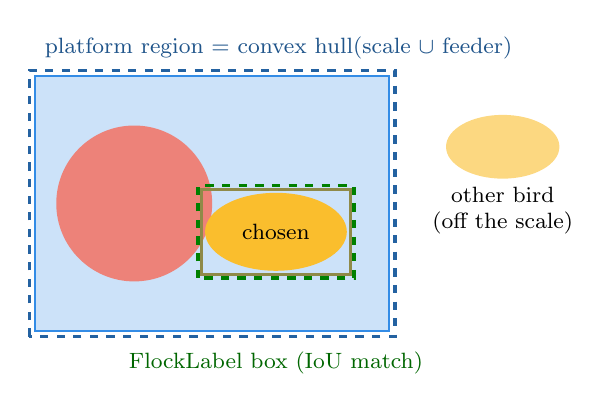
\begin{tikzpicture}[scale=0.9]
  \fill[scalec!25] (0,0) rectangle (5,3.6);
  \draw[scalec, thick] (0,0) rectangle (5,3.6);
  \draw[scalec!70!black, dashed, very thick] (-0.08,-0.08) rectangle (5.08,3.68);
  \node[scalec!60!black, font=\footnotesize, anchor=south west] at (0,3.7) {platform region = convex hull(scale $\cup$ feeder)};
  \fill[feeder!70] (1.4,1.8) circle (1.1);
  \fill[bird] (3.4,1.4) ellipse (1.0 and 0.55);
  \draw[yellow!50!black, very thick] (2.35,0.8) rectangle (4.45,2.0);
  \node[font=\footnotesize] at (3.4,1.4) {chosen};
  \fill[bird!60] (6.6,2.6) ellipse (0.8 and 0.45);
  \node[font=\footnotesize, align=center] at (6.6,1.7) {other bird\\(off the scale)};
  \draw[green!50!black, very thick, dashed] (2.3,0.75) rectangle (4.5,2.05);
  \node[green!40!black, font=\footnotesize, anchor=north] at (3.4,-0.15) {FlockLabel box (IoU match)};
\end{tikzpicture}
\caption{Bird selection: by IoU with the labelled box when there is one, otherwise by the fraction of the mask lying over the platform region.}
\label{fig:select}
\end{figure}

\begin{figure}[h]
\centering
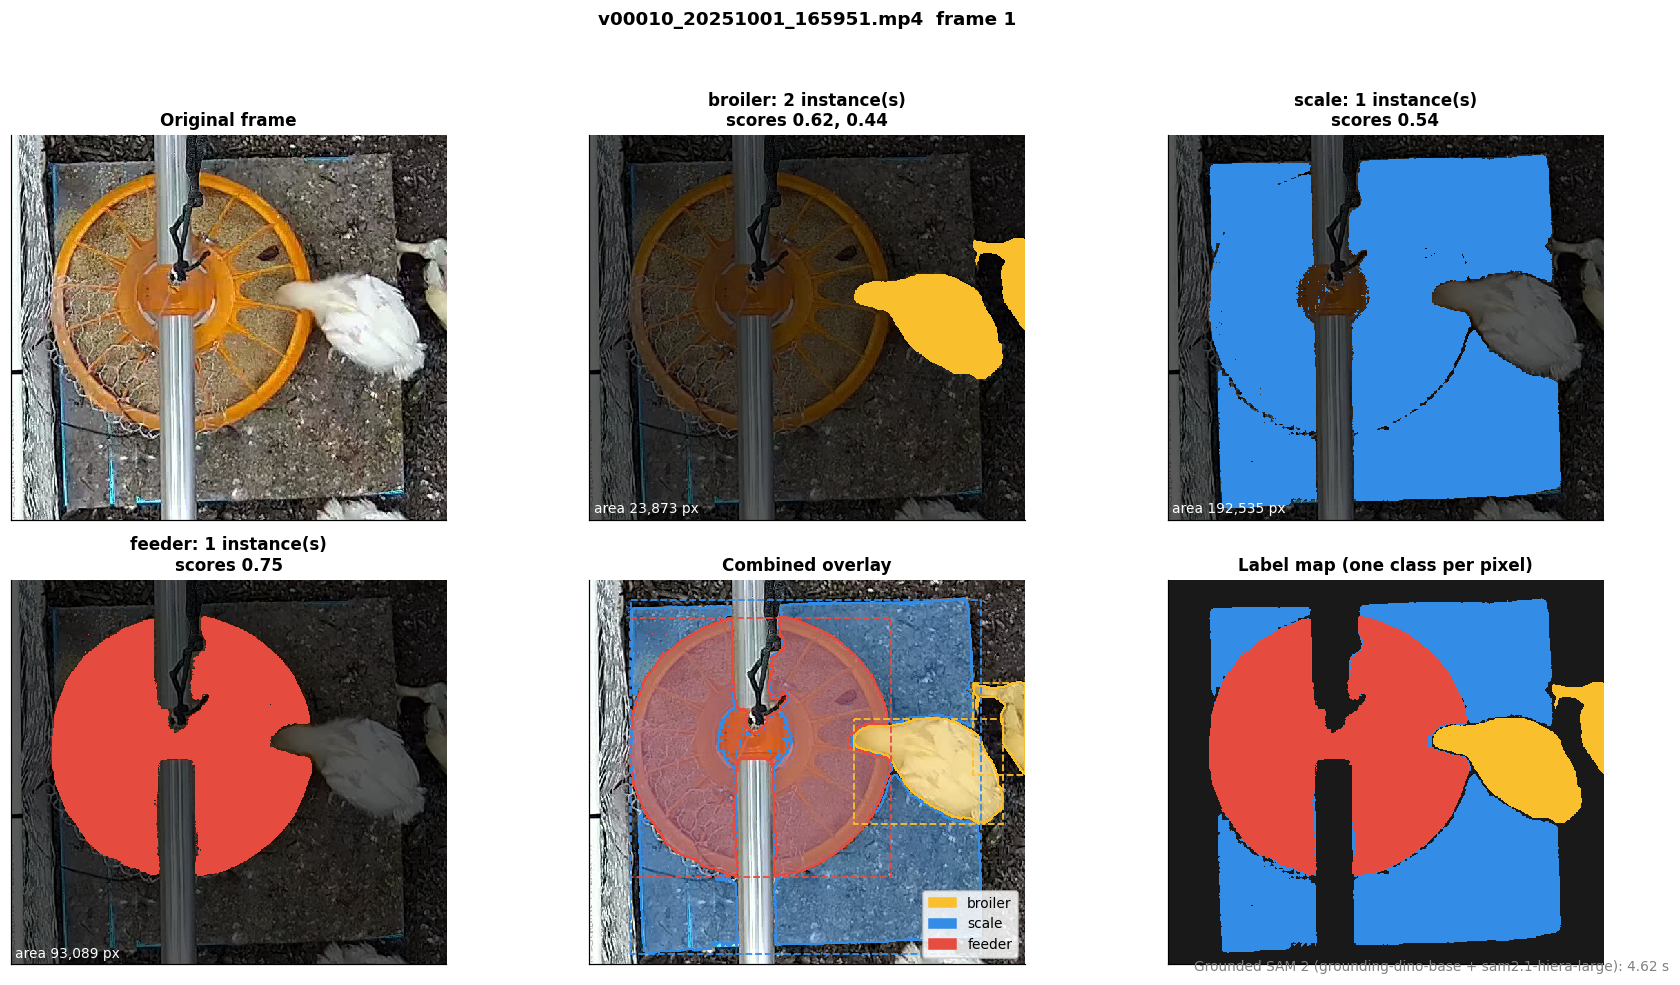
\includegraphics[width=\linewidth]{fig/real_panels.png}
\caption{Your data (event 10, frame 1): Grounded SAM 2 found two broilers, the scale and the feeder.}
\end{figure}

% =========================================================================
\section{Stage 2 -- Pixel-to-centimetre calibration}
% =========================================================================
The feeder is a circle of known diameter $D = 14\,\text{in} = 35.56$\,cm. If it measures $d_{\text{px}}$ pixels across, one pixel is
\begin{equation}
  p \;=\; \frac{D}{d_{\text{px}}}\quad [\text{cm/px}].
\end{equation}
The diameter is measured on the \emph{convex hull} of the feeder mask, because a bird often hides part of the rim. Three measurements are compared (Figure~\ref{fig:calib}):

\begin{figure}[h]
\centering
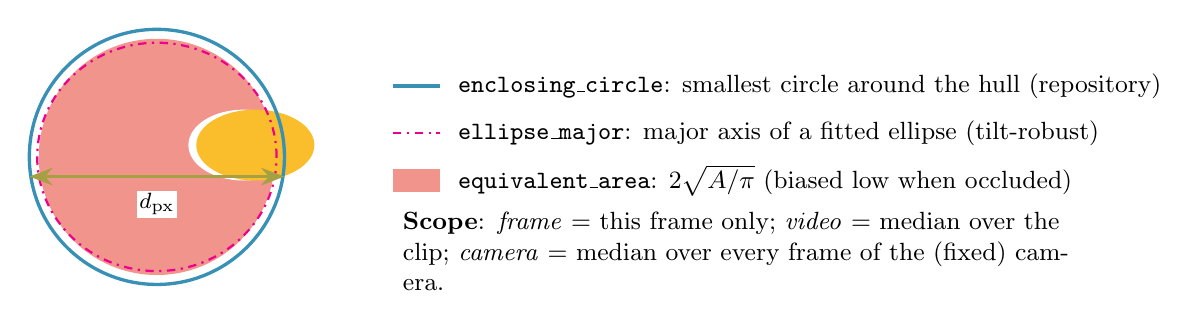
\begin{tikzpicture}[scale=1.0]
  % feeder, partly occluded
  \fill[feeder!60] (0,0) circle (1.5);
  \fill[white] (1.1,0.15) ellipse (0.7 and 0.45);
  \fill[bird] (1.25,0.15) ellipse (0.75 and 0.45);
  \draw[cyan!70!black, very thick] (0,0) circle (1.62);
  \draw[magenta, thick, dash dot] (0,0) ellipse (1.52 and 1.45);
  \draw[{Stealth}-{Stealth}, yellow!60!black, very thick] (-1.62,-0.25) -- (1.62,-0.25);
  \node[font=\footnotesize, fill=white, inner sep=1pt] at (0,-0.6) {$d_{\text{px}}$};
  % legend
  \begin{scope}[xshift=3.0cm, yshift=0.9cm, font=\small]
    \draw[cyan!70!black, very thick] (0,0) -- (0.6,0); \node[anchor=west] at (0.7,0) {\texttt{enclosing\_circle}: smallest circle around the hull (repository)};
    \draw[magenta, thick, dash dot] (0,-0.6) -- (0.6,-0.6); \node[anchor=west] at (0.7,-0.6) {\texttt{ellipse\_major}: major axis of a fitted ellipse (tilt-robust)};
    \fill[feeder!60] (0,-1.35) rectangle (0.6,-1.05); \node[anchor=west] at (0.7,-1.2) {\texttt{equivalent\_area}: $2\sqrt{A/\pi}$ (biased low when occluded)};
    \node[anchor=west, text width=9.0cm] at (0,-2.1) {\textbf{Scope}: \emph{frame} = this frame only; \emph{video} = median over the clip; \emph{camera} = median over every frame of the (fixed) camera.};
  \end{scope}
\end{tikzpicture}
\caption{Three ways to measure the feeder, and three scopes over which to take the median.}
\label{fig:calib}
\end{figure}

\begin{keybox}[Why calibration matters so much]
Volume is a length cubed, so a relative error in $p$ is \textbf{tripled} in the volume:
\[ V \propto p^{3} \;\;\Longrightarrow\;\; \frac{\Delta V}{V} \approx 3\,\frac{\Delta p}{p}. \]
In your run, events 10 and 14 got $p\approx0.0856$\,cm/px while events 8 and 16 got $p\approx0.0921$: a 7.6\% difference in $p$ that becomes a \textbf{$\approx$24\%} difference in volume for the same 450\,g bird. On the first frame the \texttt{enclosing\_circle} grabbed an outlier on the feeder mask (415.6\,px), while \texttt{ellipse\_major} gave 388.7\,px, in line with the other frames (Figure~\ref{fig:realcal}). This is why the calibration method and scope are \emph{fitted} parameters.
\end{keybox}

\begin{figure}[h]
\centering
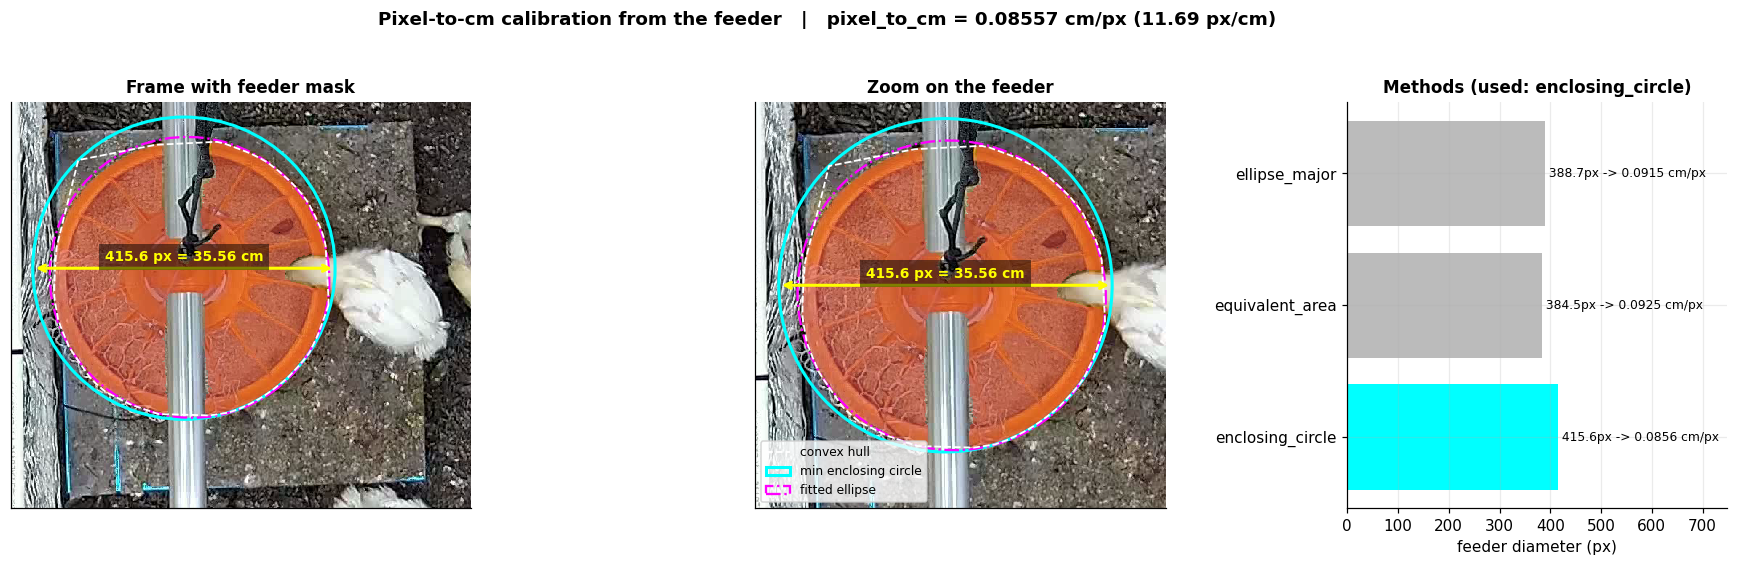
\includegraphics[width=\linewidth]{fig/real_calibration.png}
\caption{Your data: the enclosing circle (cyan) is pulled outward by a stray part of the feeder mask; the fitted ellipse (magenta) is not.}
\label{fig:realcal}
\end{figure}

% =========================================================================
\section{Stages 3--4 -- From mask to volume (the repository's slice model)}
% =========================================================================
\paragraph{Alignment.} Lines are fitted to the mask outline, and the mean of the 40th--60th percentile of their angles gives the body axis. The mask is rotated so this axis is horizontal (Figure~\ref{fig:slices}, left).

\paragraph{Slicing.} The occupied columns are split into $n$ equal groups (by default one group per pixel column). Group $i$ is treated as a \textbf{cylinder}. Its \emph{length} $w_i$ is the group width in pixels. Its \emph{diameter} $d_i$ is the mask's vertical extent at the group's middle column. Adding up the cylinders gives
\begin{equation}
  V \;=\; \sum_{i=1}^{n} \pi\Big(\frac{p\,d_i}{2}\Big)^{2} p\,w_i \;=\; \frac{\pi}{4}\,p^{3}\sum_{i=1}^{n} d_i^{2}\, w_i \quad[\text{cm}^3],
  \qquad m = \rho\,V\cdot 10^{-6}\;[\text{kg}],
  \label{eq:repo}
\end{equation}
with $\rho$ in kg/m$^3$ (repository default 900).

\begin{figure}[h]
\centering
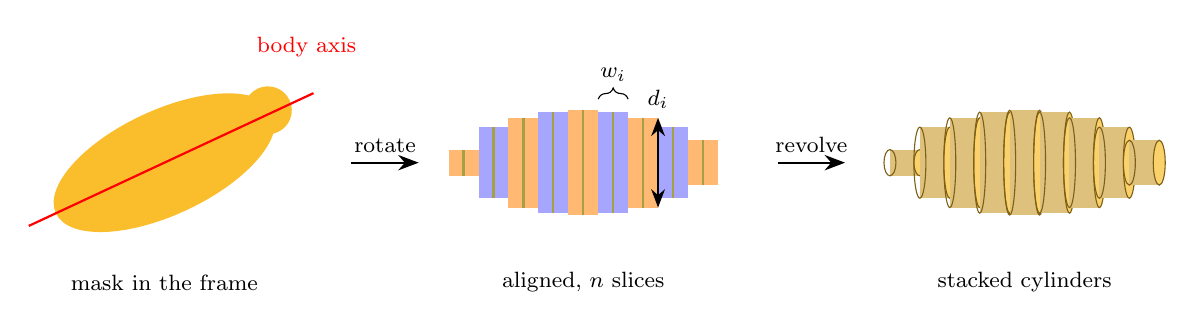
\begin{tikzpicture}[scale=0.95]
  % left: tilted mask
  \begin{scope}[rotate=25]
    \fill[bird] (0,0) ellipse (1.6 and 0.7);
    \fill[bird] (1.55,0.05) circle (0.32);
    \draw[red, thick] (-2.0,0) -- (2.2,0);
  \end{scope}
  \node[font=\footnotesize, red] at (1.9,1.55) {body axis};
  \node[font=\footnotesize] at (0,-1.6) {mask in the frame};
  \draw[arr] (2.5,0) -- (3.4,0) node[midway, above, font=\footnotesize]{rotate};
  % middle: aligned and sliced
  \begin{scope}[xshift=5.6cm]
    \foreach \x/\h [count=\k] in {-1.6/0.35,-1.2/0.95,-0.8/1.2,-0.4/1.35,0/1.4,0.4/1.35,0.8/1.2,1.2/0.95,1.6/0.6}{
      \pgfmathsetmacro{\c}{mod(\k,2)==0 ? 1 : 0}
      \ifdim\c pt=1pt \fill[blue!35] (\x-0.2,-\h/2) rectangle (\x+0.2,\h/2);
      \else \fill[orange!55] (\x-0.2,-\h/2) rectangle (\x+0.2,\h/2); \fi
      \draw[yellow!60!black, thick] (\x,-\h/2) -- (\x,\h/2);
    }
    \draw[decorate, decoration={brace, amplitude=4pt}] (0.2,0.85) -- (0.6,0.85) node[midway, above=3pt, font=\footnotesize]{$w_i$};
    \draw[{Stealth}-{Stealth}, thick] (1.0,-0.6) -- (1.0,0.6);
    \node[font=\footnotesize] at (1.0,0.85) {$d_i$};
    \node[font=\footnotesize] at (0,-1.6) {aligned, $n$ slices};
  \end{scope}
  \draw[arr] (8.2,0) -- (9.1,0) node[midway, above, font=\footnotesize]{revolve};
  % right: cylinders
  \begin{scope}[xshift=11.5cm]
    \foreach \x/\h in {-1.6/0.35,-1.2/0.95,-0.8/1.2,-0.4/1.35,0/1.4,0.4/1.35,0.8/1.2,1.2/0.95,1.6/0.6}{
      \fill[bird!80!black!60] (\x-0.2,-\h/2) rectangle (\x+0.2,\h/2);
      \draw[bird!50!black] (\x-0.2,0) ellipse (0.08 and \h/2);
      \fill[bird!70] (\x+0.2,0) ellipse (0.08 and \h/2);
      \draw[bird!50!black] (\x+0.2,0) ellipse (0.08 and \h/2);
    }
    \node[font=\footnotesize] at (0,-1.6) {stacked cylinders};
  \end{scope}
\end{tikzpicture}
\caption{The repository's volume model: rotate to the body axis, cut into slices, treat each slice as a cylinder with circular cross-section and add the volumes.}
\label{fig:slices}
\end{figure}

\begin{figure}[h]
\centering
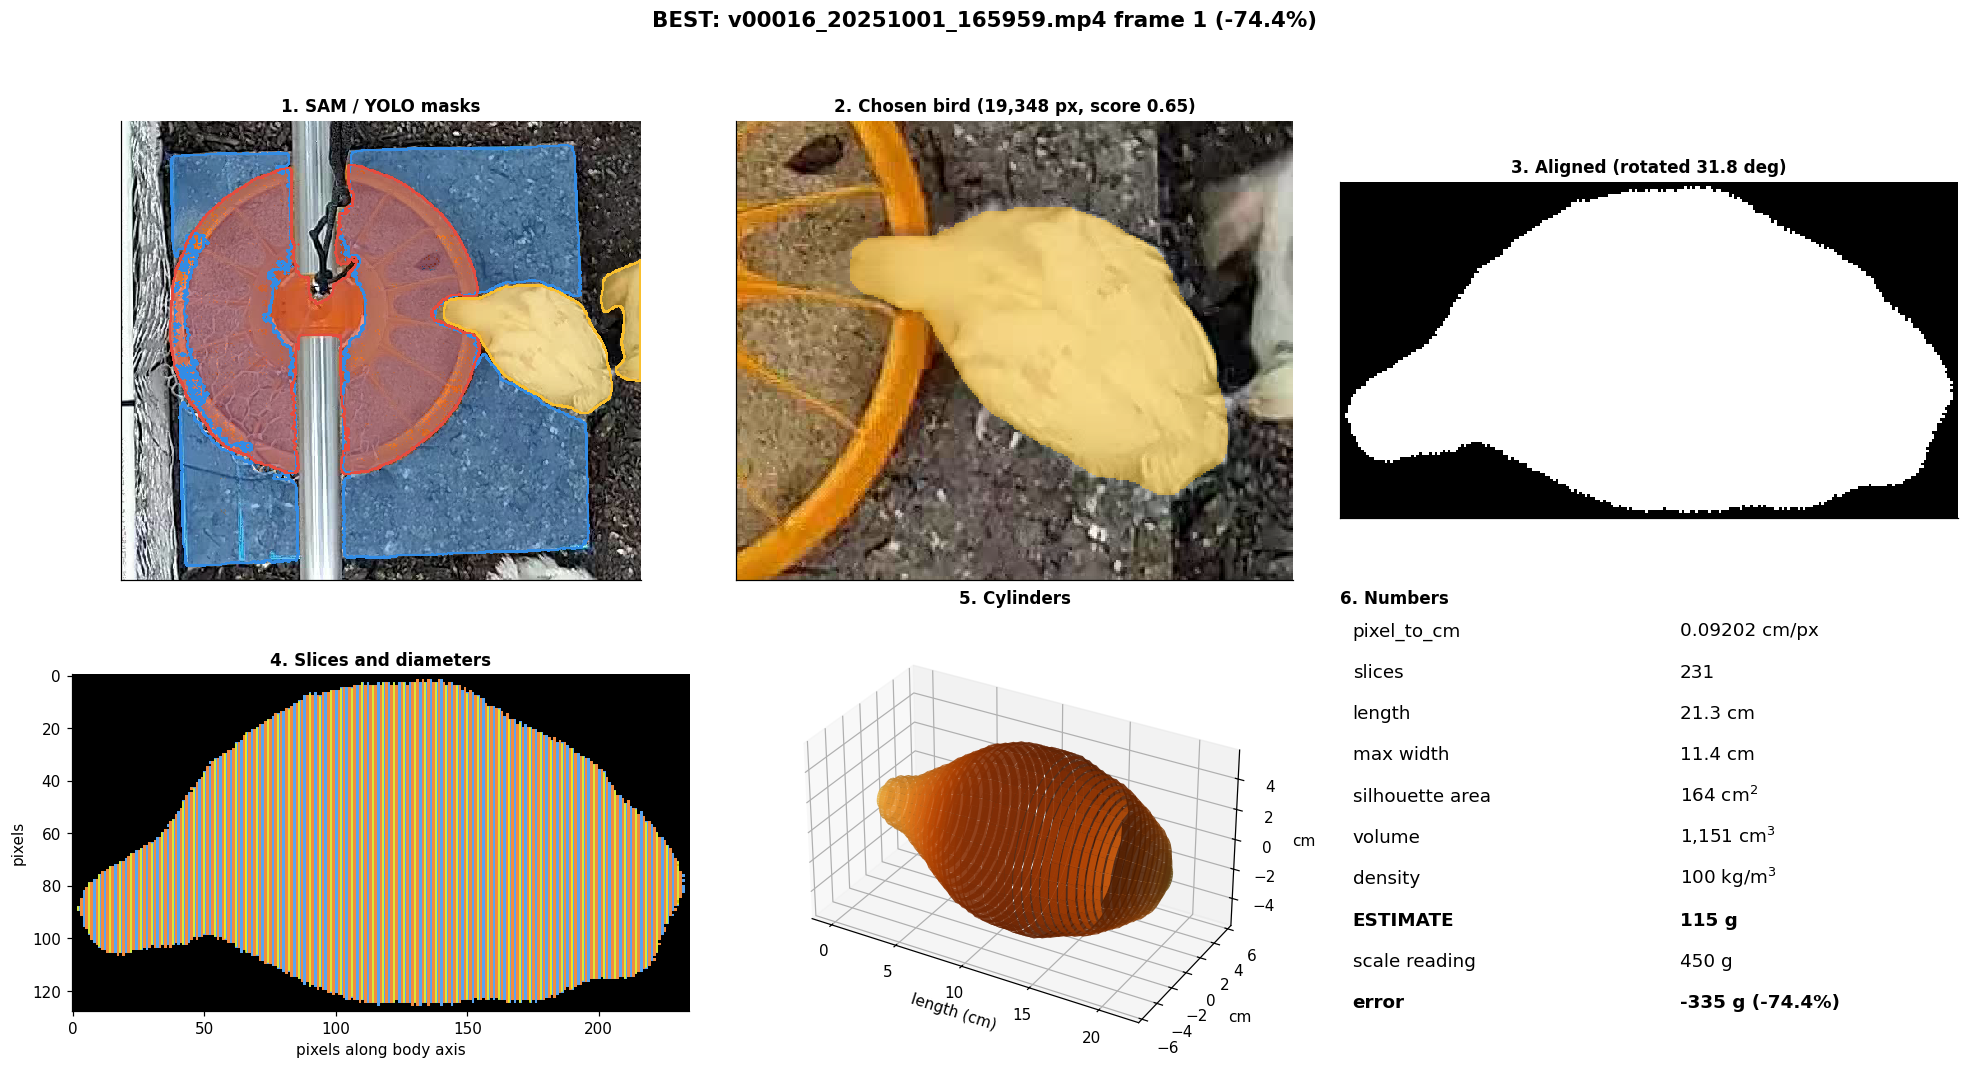
\includegraphics[width=\linewidth]{fig/real_storyboard.png}
\caption{Your data, end to end, with density 100 kg/m$^3$: volume $\approx$1{,}150\,cm$^3$ for a 450\,g bird. The \emph{implied} density (the one that would make it exact) is about 390--490 kg/m$^3$ depending on the calibration.}
\end{figure}

% =========================================================================
\section{Shortcomings of the slice model and the parameters that correct them}
% =========================================================================
\begin{enumerate}[leftmargin=*]
  \item \textbf{Mask boundary bias.} Soft feather edges make masks systematically a few pixels too large (or too small). Because $V\propto d^{2}$, a fixed pixel error is a larger \emph{fraction} of a small bird, so the bias depends on size.
  \item \textbf{Head, neck and tail.} These are sliced as solid body although they carry little mass, and how much of them is visible changes with posture.
  \item \textbf{Circular cross-section.} Depth is never measured; the model assumes depth $=$ width. A constant depth/width ratio $k$ would multiply every volume by $k$ and is therefore \emph{absorbed by the density}. It needs no separate parameter.
  \item \textbf{Calibration noise.} Error in $p$ is tripled in $V$ (previous section).
  \item \textbf{Weight not exactly proportional to volume.} Feathers, posture and body composition change with size, so mass $\propto V$ is only approximately true.
\end{enumerate}

\begin{figure}[h]
\centering
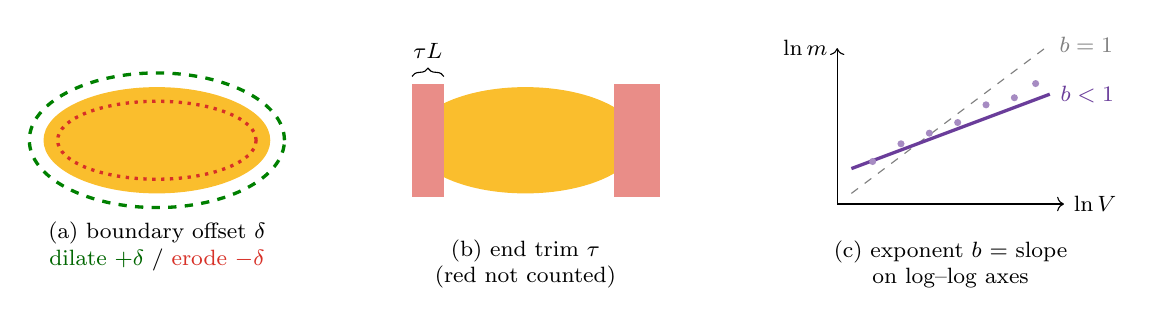
\begin{tikzpicture}[scale=0.9]
  % offset
  \begin{scope}
    \fill[bird] (0,0) ellipse (1.6 and 0.75);
    \draw[green!50!black, very thick, dashed] (0,0) ellipse (1.8 and 0.95);
    \draw[warn, very thick, dotted] (0,0) ellipse (1.4 and 0.55);
    \node[font=\footnotesize, align=center] at (0,-1.5) {(a) boundary offset $\delta$\\{\color{green!40!black}dilate $+\delta$} / {\color{warn}erode $-\delta$}};
  \end{scope}
  % trim
  \begin{scope}[xshift=5.2cm]
    \fill[bird] (0,0) ellipse (1.6 and 0.75);
    \fill[bird] (1.55,0.05) circle (0.32);
    \fill[warn!55] (-1.6,-0.8) rectangle (-1.15,0.8);
    \fill[warn!55] (1.25,-0.8) rectangle (1.9,0.8);
    \fill[white] (-1.9,-0.85) rectangle (-1.6,0.85);
    \draw[decorate, decoration={brace, amplitude=3pt}] (-1.6,0.9) -- (-1.15,0.9) node[midway, above=3pt, font=\footnotesize]{$\tau L$};
    \node[font=\footnotesize, align=center] at (0,-1.75) {(b) end trim $\tau$\\(red not counted)};
  \end{scope}
  % exponent
  \begin{scope}[xshift=9.6cm, yshift=-0.9cm]
    \draw[->] (0,0) -- (3.2,0) node[right, font=\footnotesize]{$\ln V$};
    \draw[->] (0,0) -- (0,2.2) node[left, font=\footnotesize]{$\ln m$};
    \draw[gray, dashed] (0.2,0.15) -- (3.0,2.25) node[right, font=\footnotesize]{$b=1$};
    \draw[teach, very thick] (0.2,0.5) -- (3.0,1.55) node[right, font=\footnotesize]{$b<1$};
    \foreach \x/\y in {0.5/0.6,0.9/0.85,1.3/1.0,1.7/1.15,2.1/1.4,2.5/1.5,2.8/1.7}{\fill[teach!60] (\x,\y) circle (0.05);}
    \node[font=\footnotesize, align=center] at (1.6,-0.85) {(c) exponent $b$ = slope\\on log--log axes};
  \end{scope}
\end{tikzpicture}
\caption{Three of the corrections: (a) boundary offset, (b) end trim, (c) size exponent.}
\label{fig:corrections}
\end{figure}

% =========================================================================
\section{One mass equation}
% =========================================================================
All corrections are combined into a single equation:

\begin{keybox}[The fitted mass equation]
\[
  \boxed{\;\hat m \;=\; a\left[\frac{\pi}{4}\,p_c^{3}\sum_{i\in S_\tau}\Big(d_i^{(\delta)}\Big)^{2} w_i\right]^{b} \;=\; a\,V(\delta,\tau,n,c)^{\,b}\;}
\]
\begin{tabular}{@{}l>{\raggedright\arraybackslash}p{8.6cm}>{\raggedright\arraybackslash}p{4.2cm}@{}}
\toprule
symbol & meaning & how it is fitted\\
\midrule
$\delta$ & boundary offset (px): mask dilated ($+$) or eroded ($-$) & grid search\\
$\tau$ & fraction of body length trimmed at each end & grid search\\
$n$ & number of slices ($S_\tau$ = slices left after trimming) & grid search\\
$c$ & calibration method $\times$ scope, giving $p_c$ & grid search\\
$b$ & size exponent (1 = weight proportional to volume) & closed form, ridge towards 1\\
$a$ & scale; for $b=1$, $\rho = a\cdot10^{6}$ kg/m$^3$ & closed form\\
\bottomrule
\end{tabular}
\end{keybox}

With $\delta=0,\ \tau=0,\ n=\text{per column},\ c=\text{enclosing circle},\ b=1$ the equation \emph{is} the repository model (\ref{eq:repo}) with $\rho=a\cdot10^6$.

\paragraph{What can be learned from which data.} Any factor that scales every bird by the same amount is indistinguishable from $a$: a constant depth ratio, a constant perspective correction, or a fixed calibration bias. Only settings that change birds \emph{relative to each other} can be learned. The exponent $b$ needs birds of \emph{different} weights. If the event weights vary by less than 5\% (coefficient of variation), $b$ is fixed at 1 automatically. Your current four events are all 450\,g, so for now the data can fit $a$ (the density) and the settings that make repeated measurements of the same bird agree ($\delta,\tau,n,c$), but not $b$.

% =========================================================================
\section{Fitting the parameters}
% =========================================================================
\subsection{$a$ and $b$ in closed form}
Taking logarithms turns the equation into a straight line, $\ln m = \ln a + b\ln V$. Errors are then relative, which suits weights spanning a wide range. Each frame $j$ gets weight $w_j = 1/(\text{frames in its event})$, so every event counts equally, and $b$ is pulled gently towards 1 by a ridge penalty of strength $\lambda=r\sum_j w_j$ (default $r=0.1$):
\begin{equation}
  \min_{\alpha,\,b}\ \sum_j w_j\big(\ln m_j-\alpha-b\ln V_j\big)^{2}+\lambda\,(b-1)^{2},\qquad a=e^{\alpha}.
\end{equation}
Setting the derivatives to zero gives a $2\times2$ linear system, solved exactly:
\begin{equation}
\begin{pmatrix}\sum w & \sum w x\\ \sum w x & \sum w x^{2}+\lambda\end{pmatrix}
\begin{pmatrix}\alpha\\ b\end{pmatrix}=
\begin{pmatrix}\sum w y\\ \sum w x y+\lambda\end{pmatrix},\qquad x=\ln V,\ y=\ln m.
\end{equation}
With $b$ fixed at 1 this reduces to a weighted geometric mean: $a=\exp\!\big(\sum w(y-x)/\sum w\big)$.

\subsection{The discrete settings by grid search}
Every combination of $\delta\in\{-6,\dots,6\}$, $\tau\in\{0,\dots,0.15\}$, $n\in\{\text{per column},5,\dots,30\}$, the three calibration methods and the three scopes, with $b$ fixed or free, is tried (typically 1{,}000--5{,}000 combinations). The volumes are computed once in pixel units and multiplied by $p_c^3$ afterwards, so the search takes seconds. If two combinations have the same error, the simpler one is kept (offset~0, no trim, $b=1$).

\subsection{Scoring: leave-one-event-out cross-validation}
A setting must be judged on events it was \emph{not} fitted to. With $E$ events, each event is held out in turn: $a,b$ are fitted on the other $E-1$, and the held-out event is predicted (Figure~\ref{fig:loeo}). The score compares the \emph{median} prediction with the \emph{median} scale reading of each event:
\begin{equation}
  \text{RMSE}_{\text{CV}}=\sqrt{\frac{1}{E}\sum_{e=1}^{E}\Big(\operatorname{median}_{j\in e}\hat m_j^{(-e)}-\operatorname{median}_{j\in e}m_j\Big)^{2}}.
\end{equation}
Whole events are held out, never single frames: frames of one weighing are near-duplicates, so mixing them would leak the answer.

\begin{figure}[h]
\centering
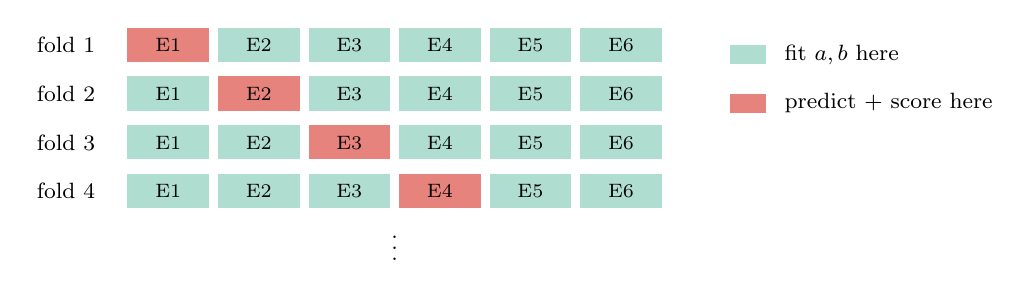
\begin{tikzpicture}[x=1.15cm,y=0.62cm]
  \foreach \r in {1,...,4}{
    \node[font=\footnotesize, anchor=east] at (0.3,-\r) {fold \r};
    \foreach \c in {1,...,6}{
      \pgfmathtruncatemacro{\test}{\c==\r ? 1 : 0}
      \ifnum\test=1 \fill[warn!60] (\c-0.45,-\r-0.35) rectangle (\c+0.45,-\r+0.35);
      \else \fill[stud!35] (\c-0.45,-\r-0.35) rectangle (\c+0.45,-\r+0.35); \fi
      \node[font=\scriptsize] at (\c,-\r) {E\c};
    }
  }
  \node[font=\footnotesize] at (3.5,-5.0) {$\vdots$};
  \fill[stud!35] (7.2,-1.4) rectangle (7.6,-1.0); \node[font=\footnotesize, anchor=west] at (7.7,-1.2) {fit $a,b$ here};
  \fill[warn!60] (7.2,-2.4) rectangle (7.6,-2.0); \node[font=\footnotesize, anchor=west] at (7.7,-2.2) {predict + score here};
\end{tikzpicture}
\caption{Leave-one-event-out cross-validation: every event is predicted by a model that never saw it.}
\label{fig:loeo}
\end{figure}

\subsection{Nested cross-validation: an honest error for the whole procedure}
Choosing the best of thousands of settings by their cross-validated error is itself a form of fitting. With few events, the winning setting may simply have been lucky, so its CV error is optimistic (\emph{selection bias}). \textbf{Nested} cross-validation repeats the \emph{entire search} without each event and only then predicts that event (Figure~\ref{fig:nested}). Its error is the number to report. Comparing the settings chosen in different folds also shows whether the data really determine them.

\begin{figure}[h]
\centering
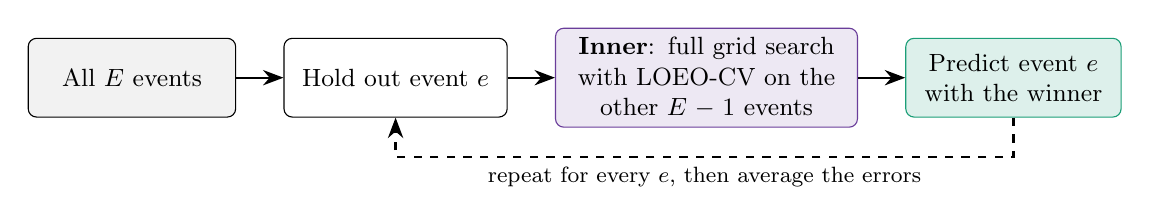
\begin{tikzpicture}[node distance=0.4cm and 0.6cm]
  \node[data, text width=2.4cm] (all) {All $E$ events};
  \node[box, right=of all, text width=2.6cm] (hold) {Hold out event $e$};
  \node[model, right=of hold, text width=3.6cm] (search) {\textbf{Inner}: full grid search\\with LOEO-CV on the\\other $E-1$ events};
  \node[res, right=of search, text width=2.5cm] (pred) {Predict event $e$\\with the winner};
  \draw[arr] (all) -- (hold); \draw[arr] (hold) -- (search); \draw[arr] (search) -- (pred);
  \draw[arr, dashed] (pred.south) -- ++(0,-0.5) -| node[pos=0.25, below, font=\footnotesize]{repeat for every $e$, then average the errors} (hold.south);
\end{tikzpicture}
\caption{Nested cross-validation.}
\label{fig:nested}
\end{figure}

\begin{figure}[h]
\centering
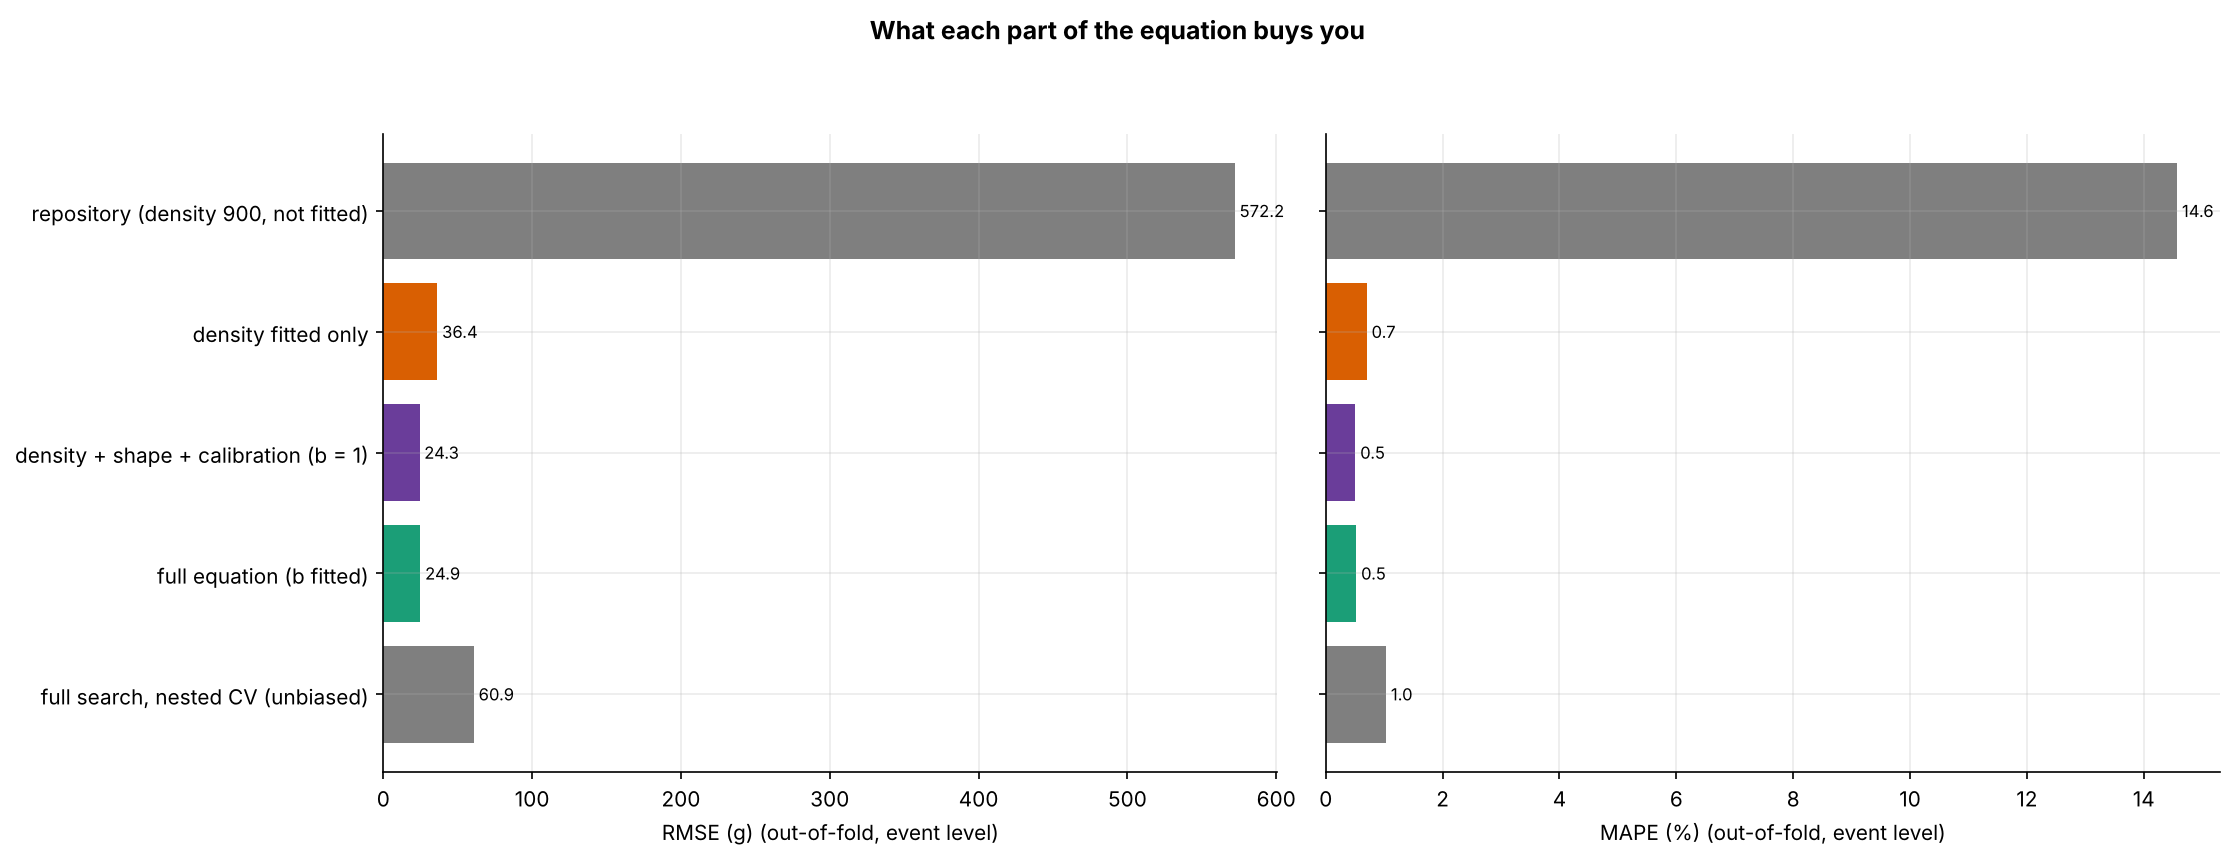
\includegraphics[width=\linewidth]{fig/demo_comparison.png}
\caption{\emph{Demo data} (six synthetic events). Fitting the density removes almost all of the repository's error; shape and calibration settings help a little more. The \textbf{nested} error, however, is higher than ``density fitted only'': with six events the search over thousands of settings partly fits noise. With few events, prefer the simpler model unless the nested error says otherwise.}
\end{figure}

\begin{figure}[h]
\centering
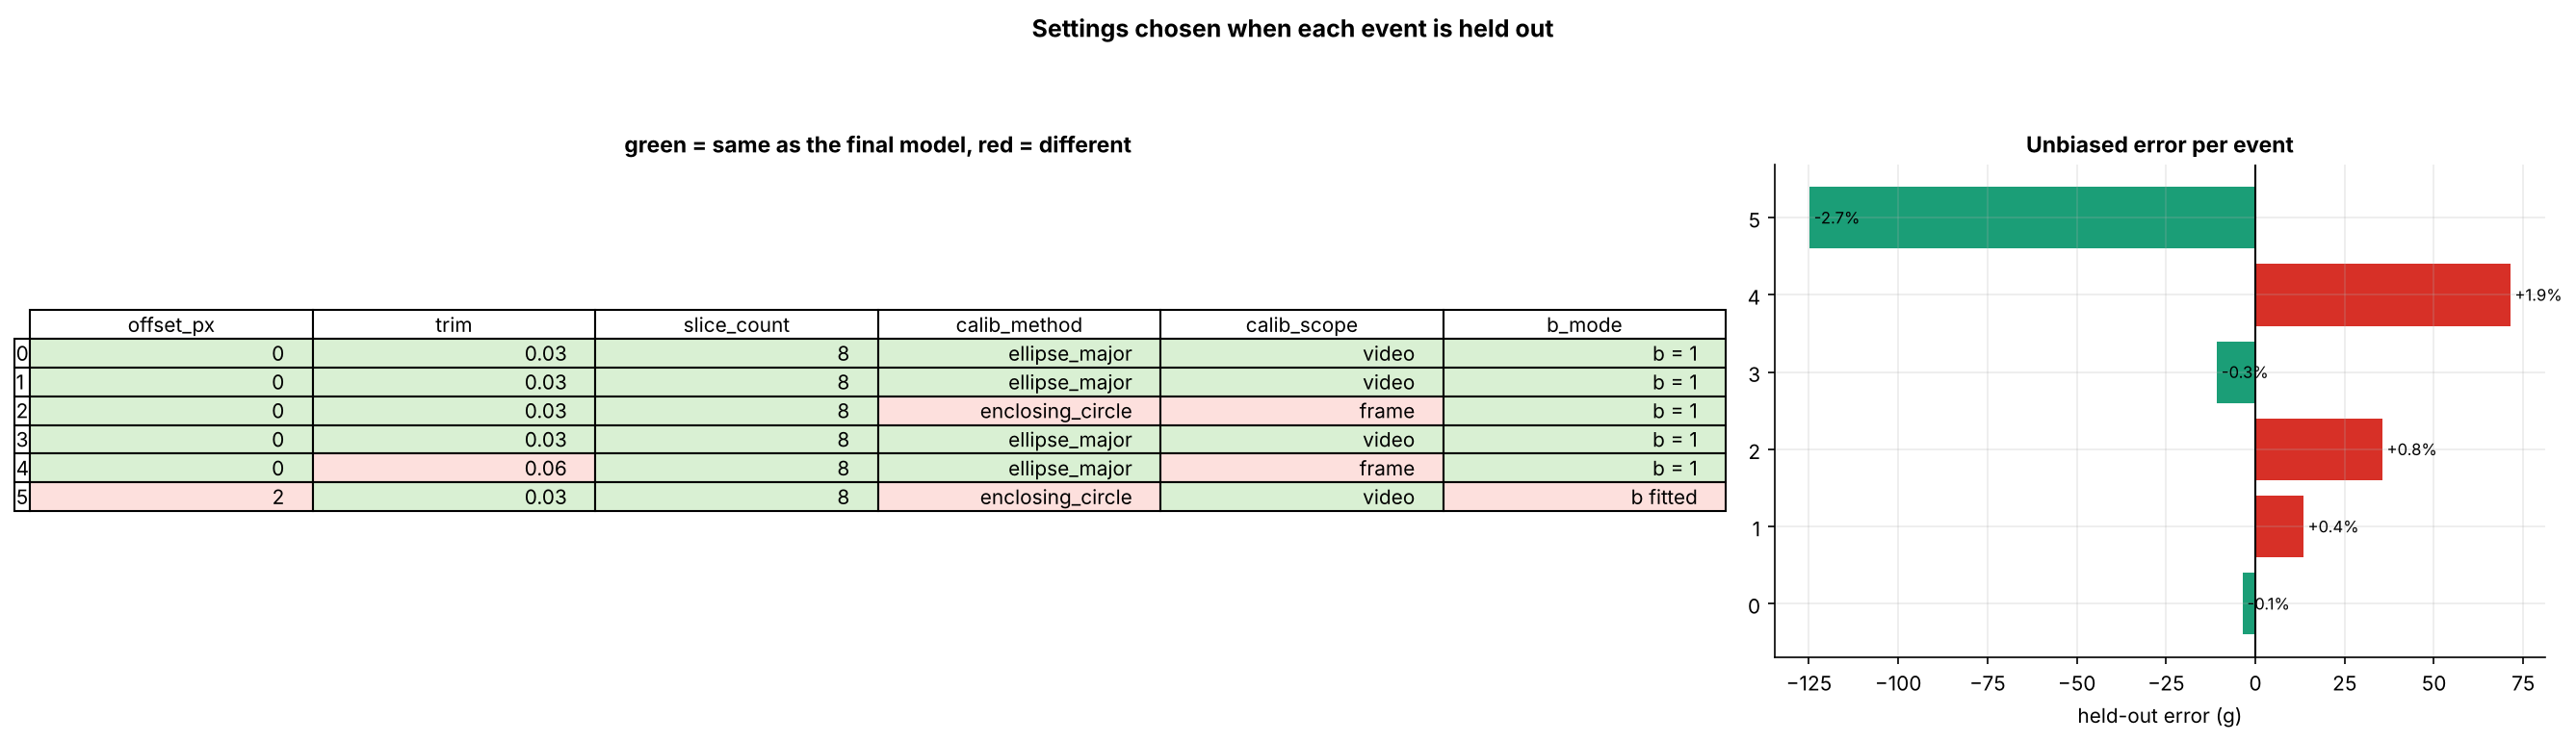
\includegraphics[width=\linewidth]{fig/demo_nested.png}
\caption{\emph{Demo data}: the settings chosen without each event. Mostly stable (green); where they differ (red) the data cannot pin the setting down.}
\end{figure}

\begin{figure}[h]
\centering
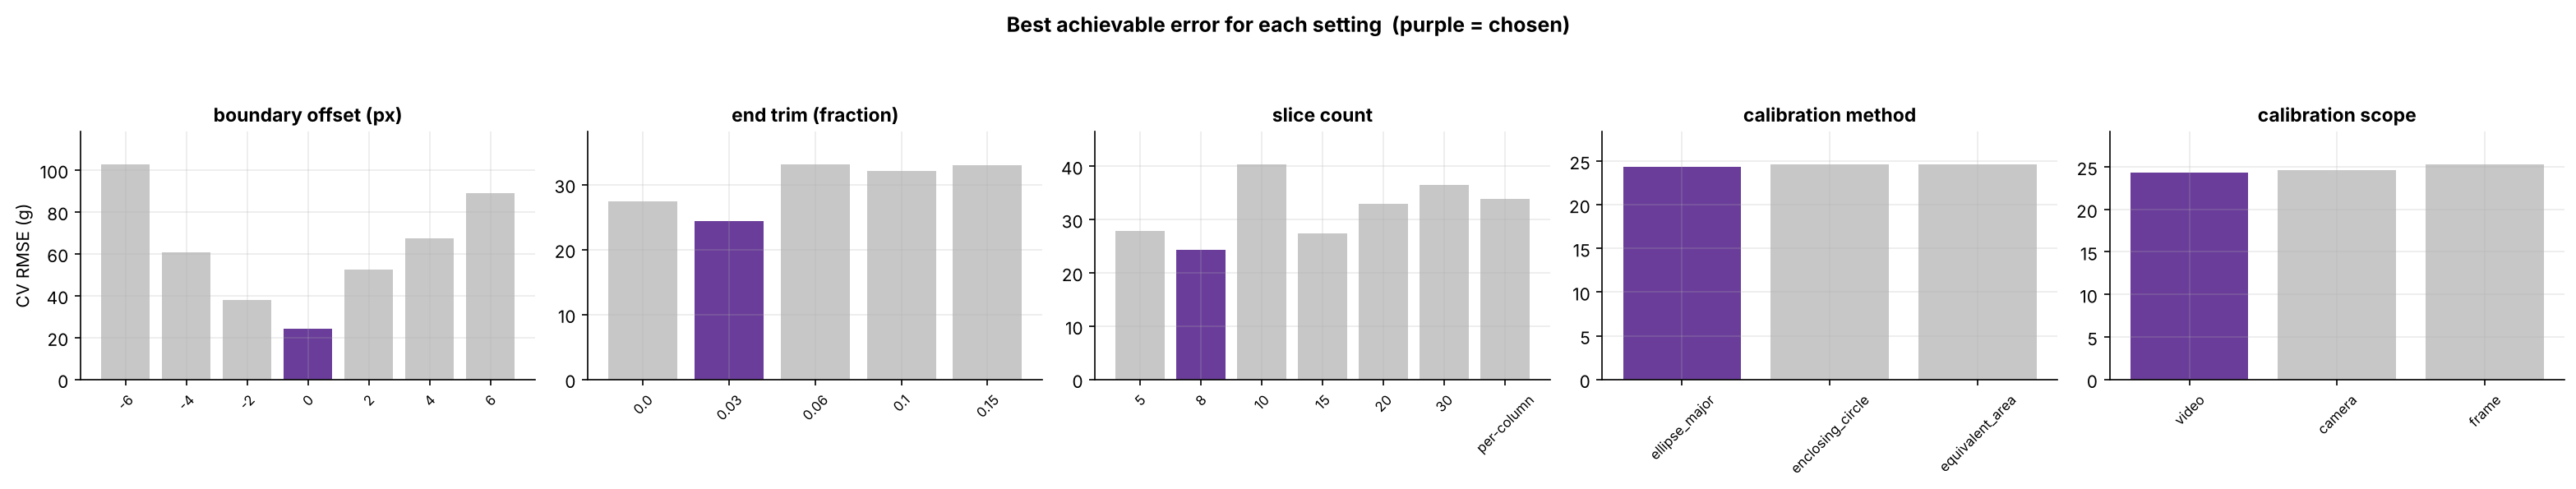
\includegraphics[width=\linewidth]{fig/demo_sensitivity.png}
\caption{\emph{Demo data}: best cross-validated error reachable for each value of each setting. A clear dip means the setting matters; a flat panel means keep its simplest value.}
\end{figure}

% =========================================================================
\section{The most accurate density}
% =========================================================================
With $b=1$ the equation is the physical model, and $a$ is a density: $\rho=a\cdot10^6$ kg/m$^3$. The package reports
\begin{itemize}[nosep]
  \item the density fitted on all events (with the chosen $\delta,\tau,n,c$);
  \item the range of densities obtained when each event is left out in turn (stability);
  \item a 95\% bootstrap interval from resampling whole events 2{,}000 times;
  \item the frame-by-frame \emph{implied} density $m_j/V_j$, which shows the scatter one density must cover.
\end{itemize}

\begin{notebox}[A density belongs to its settings]
The fitted density is only meaningful together with the shape and calibration settings it was fitted with. Trimming 10\% of the length or eroding the mask removes volume, so the density must rise to compensate. In one demo run it went from about 780 (repository settings) to about 990 (offset $-2$\,px, trim 10\%). Always quote the density with its settings. The notebook writes both to \texttt{mass\_model.json}.
\end{notebox}

\begin{figure}[h]
\centering
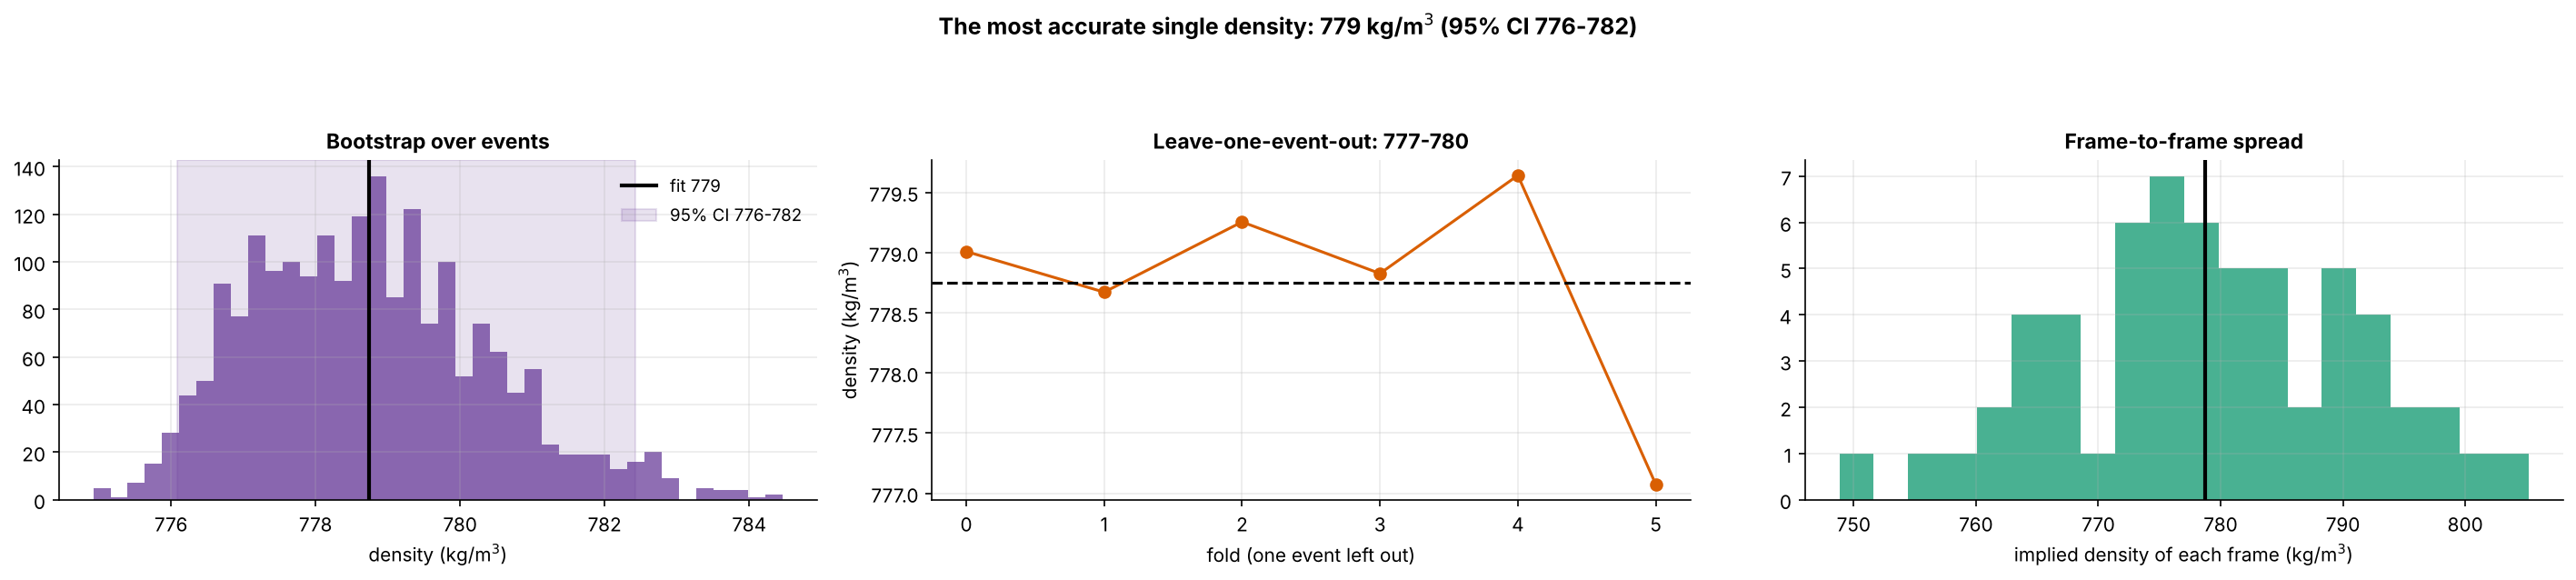
\includegraphics[width=\linewidth]{fig/demo_density.png}
\caption{\emph{Demo data}: density estimate with bootstrap interval, leave-one-event-out stability and the per-frame implied density.}
\end{figure}

% =========================================================================
\section{Knowledge distillation for the Raspberry Pi}\label{sec:distill}
% =========================================================================
The teachers are far too large for a Raspberry Pi, so Notebook~2 transfers their knowledge to a small student (Figure~\ref{fig:distill}). This is \emph{response-based} distillation: the teacher's masks are the student's training labels. The student is then judged twice: by mask IoU against the teacher, and, more importantly, by the weight error when its masks go through the same equation.

\begin{figure}[h]
\centering
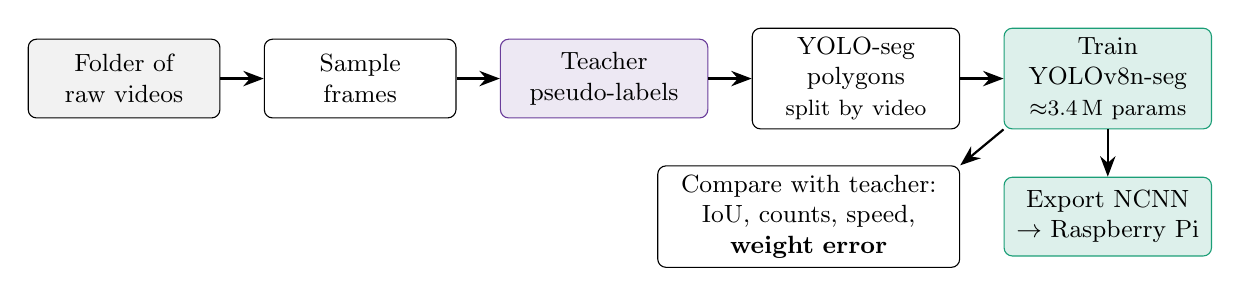
\begin{tikzpicture}[node distance=0.45cm and 0.55cm]
  \node[data, text width=2.2cm] (v) {Folder of\\raw videos};
  \node[box, right=of v, text width=2.2cm] (s) {Sample\\frames};
  \node[model, right=of s, text width=2.4cm] (t) {Teacher\\pseudo-labels};
  \node[box, right=of t, text width=2.4cm] (y) {YOLO-seg\\polygons\\{\footnotesize split by video}};
  \node[res, right=of y, text width=2.4cm] (st) {Train\\YOLOv8n-seg\\{\footnotesize $\approx$3.4\,M params}};
  \node[res, below=0.6cm of st, text width=2.4cm] (pi) {Export NCNN\\$\to$ Raspberry Pi};
  \node[box, left=of pi, text width=3.6cm] (cmp) {Compare with teacher:\\IoU, counts, speed,\\\textbf{weight error}};
  \draw[arr] (v) -- (s); \draw[arr] (s) -- (t); \draw[arr] (t) -- (y); \draw[arr] (y) -- (st);
  \draw[arr] (st) -- (pi); \draw[arr] (st.south west) -- (cmp.north east);
\end{tikzpicture}
\caption{Distillation in Notebook 2.}
\label{fig:distill}
\end{figure}

% =========================================================================
\section{What your current data can and cannot tell you}
% =========================================================================
\begin{tabular}{@{}>{\raggedright\arraybackslash}p{4.6cm}>{\raggedright\arraybackslash}p{10.4cm}@{}}
\toprule
\textbf{Observation (your run)} & \textbf{Consequence}\\
\midrule
4 events, 8 labelled frames & Leave-one-event-out uses 3 events to fit and 1 to test; nested CV uses 2--3 inside. Treat any choice of $\delta,\tau,n$ as provisional.\\
All events weigh 450\,g & $b$ cannot be learned and stays at 1. $R^2$ is undefined. The density is learned for 450\,g birds only.\\
Two calibration clusters (0.0856 vs 0.0921 cm/px) & The main source of disagreement between events. Fitting $c$ (e.g.\ \texttt{ellipse\_major} or camera scope) should reduce it.\\
Implied density 390--490 kg/m$^3$ & Well below tissue density ($\approx$1{,}050), as expected: the circular cross-section over-states depth, and the mask includes loose feathers.\\
\bottomrule
\end{tabular}

\paragraph{Recommendations.}
\begin{enumerate}[nosep]
  \item Label more weighing \textbf{events} (aim for 20 or more) rather than more frames per event; 10--40 frames per event is plenty.
  \item Cover a \textbf{range of weights} (e.g.\ several ages, 0.4--3\,kg) so that $b$ becomes identifiable and the density is not tied to one size.
  \item Report the \textbf{nested} cross-validated error, together with the fitted equation and its settings.
  \item If nested CV prefers the simple model, use \emph{density + calibration only} until more data arrive.
\end{enumerate}

\appendix
\section{Symbols}
\begin{tabular}{@{}ll@{}}
\toprule
$p$, $p_c$ & centimetres per pixel (from the feeder; $c$ = method $\times$ scope)\\
$D$ & feeder diameter, 35.56\,cm\\
$d_i$, $w_i$ & diameter and length (pixels) of slice $i$\\
$n$, $S_\tau$ & slice count; slices kept after trimming fraction $\tau$ at each end\\
$\delta$ & mask boundary offset in pixels\\
$V$ & adjusted slice volume (cm$^3$)\\
$a$, $b$ & scale and exponent of $\hat m=aV^b$; $\rho=a\cdot10^6$ when $b=1$\\
$E$ & number of weighing events\\
\bottomrule
\end{tabular}

\end{document}
